\documentclass[letterpaper, final]{book}
\makeindex

%%%%%%%%%%%%%%%%%%%%%%
% Packages and library
%%%%%%%%%%%%%%%%%%%%%%

% Langue
\usepackage[french]{babel}

% Contenu
\usepackage{amsmath}
\usepackage{pgfplots}
\usepackage{pdfpages}
\usepackage[url=false]{biblatex}
\usepackage{makeidx}

% Mise en page
\usepackage{geometry}
\usepackage{caption}
\usepackage{framed}
\usepackage{marginnote}
\usepackage{hyperref}
\usepackage{fancyhdr}
\usepackage{tocloft}
\usepackage[toc, title]{appendix}
\usepackage[outercaption, wide]{sidecap}
\usepackage[framed]{ntheorem}
\usepackage[nobottomtitles]{titlesec}

% Paquets personnels

\usepackage{logochum}
\usepackage{vdr}
\usepackage{horaire}
\usepackage{titlepage2}
\usepackage{exercice}

% Librairies

\usetikzlibrary{backgrounds}
\usetikzlibrary{external}
\usetikzlibrary{positioning}
\usetikzlibrary{matrix}
\usepgfplotslibrary{groupplots}

%%%%%%%%%%%%%%%%%%%%%%
% Configurations
%%%%%%%%%%%%%%%%%%%%%%

\hypersetup{
	pdfusetitle,
	hidelinks,
	pdfencoding=unicode
}

\geometry{
	includeall,
	margin=0.8in,
	marginparwidth=2in,
	marginparsep=0.3in
}
\pretolerance=1000

% Headder and footer
\def\headrulewidth{0pt}
\pagestyle{fancy}
\addtolength{\headwidth}{\marginparwidth}
\addtolength{\headwidth}{\marginparsep}

\tikzset{external/only named=true}
\tikzsetexternalprefix{fig-pdf/}

\setlength{\parskip}{.7em}
\def\arraystretch{1.5}
\setcounter{tocdepth}{1}
%\setsecnumdepth{subsection}
\definecolor{shadecolor}{gray}{0.85}

\DefineBibliographyStrings{french}{in={dans}}
\AtBeginDocument{\renewcommand{\listfigurename}{Liste des figures}}

%%%%%%%%%
% Macro
%%%%%%%%%

\def\param#1{{\small \uppercase{#1}}}

\def\knobshow#1{%
	\marginpar{%
		\centering
		\begin{tikzpicture} \pic [scale=1.5] {labeleb=#1}; \end{tikzpicture}}}

\def\protochum#1{#1 \logochum[height=11pt]}

\theoremstyle{nonumberbreak}
\newframedtheorem{auchum}{Au CHUM...}

\newenvironment{fullwidth}{
\newgeometry{
	includeall,
	margin=0.8in,
	marginparwidth=0in,
	marginparsep=0in
}
}{
\restoregeometry
}

\def\ie{$i\, \colon e$}
\def\fio{$FiO_2$}

\addbibresource{bibliography.bib}
\tikzexternalize
%\includeonly{chap/chapSurveillance}

\title{Ventilation diffusive convective}
\subtitle{\emph{Opérer} et \emph{comprendre} le ventilateur VDR-4}
\author{Nicolas Blais St-Laurent}
\date{2020}
\titlegraphic{\includegraphics{titlepage/cover}}

\hypersetup{
	pdftitle=Ventilation diffusive convective,
	pdfauthor=Nicolas Blais St-Laurent
}

\begin{document}

%%%%%%%%%%%%%%
% Frontmatter
%%%%%%%%%%%%%%
\frontmatter
\maketitle

\cleardoublepage
\tableofcontents
%\listoftables
\clearpage
\listoffigures
%\listofexercices

%%%%%%%%%%%%%%
% Mainmatter
%%%%%%%%%%%%%%

\mainmatter
\chapter{Introduction}

Le VDR-4 est un appareil de ventilation à haute fréquence conçu au cours des
années 1980\cite{Vienne2008} par l'inventeur américain Forest Morton Bird.  Il a été conçu en
tant qu'appareil de ventilation universel, capable de ventiler adéquatement
n'importe quel poumon humain, sain ou gravement malade, de la clientèle
néonatale à la clientèle adulte.  Son développement a été motivé par le constat
que la ventilation mécanique en pression positive conventionnelle (c'est-à-dire
basée sur un volume courant et une fréquence physiologiques) était peu adaptée
à la ventilation d'un patient présentant une pathologie pulmonaire inhomogène
(MPOC, pneumonie, brûlure d'inhalation, SDRA, etc.).

Outre le type singulier de ventilation qu'il délivre \footnote{Voir
section~\ref{sec:particularite}}, le VDR-4 se distingue aussi par son
fonctionnement entièrement pneumatique. Ceci lui confère l'avantage de
fonctionner indépendament de toute alimentation électrique. En contrepartie,
l'appareil a des capacités de monitorage très limitées, et une interface
utilisateur peu conviviale.

\section{Vocabulaire}

\begin{description}
	\item[Convection:] Déplacement d'un volume de gaz. Lors de la ventilation
	<<conventionnelle>>, les échanges gazeux entre le circuit du ventilateur et
	les bronchioles terminales se font par convection\cite{West2017}. On peut donc parler de
		ventilation \em{convective}.  
	\item [Diffusion:] Déplacement des molécules d'un gaz à l'intérieur d'un mélange gazeux. Les molécules d'un gaz diffusent en suivant leur gradient de concentration.
	\item [Hertz:] Unité de mesure de fréquence correspondant à un cycle par seconde ou soixante cycles par minute.
	\item [Iatrogène:] Causé par la thérapie.
	\item [Percussion:] Bref jet de gaz à haute vélocité.
	\item [Pression motrice:] Dans un contexte de ventilation par VDR-4, on désigne pression motrice la différence entre la pression moyenne à l'inspiration et la pression moyenne à l'expiration.
	\item [Pression partielle:] Pression exercée par les molécules d'un gaz à l'intérieur d'un mélange gazeux.
\end{description}

\section{Notions de ventilation à haute fréquence}

Ce qui caractérise la ventilation à haute fréquence est l'administration de
volumes courants inférieurs au volume de l'espace mort anatomique du patient.
Les échanges gazeux entre les alvéoles et le circuit de ventilation s'y font
selon un ensemble de mécanismes différents. À ce jour, l'influence respective
de chacun de ces mécanismes reste encore à élucider\cite{Pillow2005}.

\subsection{Oxygénation lors de la ventilation à haute fréquence}

Les facteurs influençant l'oxygénation lors de la ventilation à haute fréquence
sont, à toute fin pratique, les mêmes que pour la ventilation convective.

Dans l'absolu, l'oxygénation du sang est proportionnelle à la pression
partielle d'oxygène dans les alvéoles. Les trois principales variables
influençant cette pression partielle sont: la concentration d'oxygène dans
l'air insufflé, la pression alvéolaire moyenne, la concentration alvéolaire de
gaz carbonique.

\subsection{Relation fréquence-volume-ventilation}

Ce qui limite les volumes courants en ventilation à haute fréquence est le peu
de temps disponible pour chaque cycle respiratoire. Ce temps est d'autant plus
court que la fréquence est élevée. 
\marginpar{%
$$ {T_{cycle}}{(s)} = \frac{60}{Freq{(/m)}}$$%
}
En conséquence, une diminution de la fréquence entrainera une augmentation du
volume courant en laissant plus de temps à la pression pour s'équilibrer entre
le circuit et les alvéoles. Inversement, une augmentation de la fréquence
entrainera une diminution du volume courant.

Ainsi, en ventilation à haute fréquence, une diminution de la fréquence
favorise une plus grande élimination du $CO_2$.

Il a été démontré que la fréquence est un paramètre très important pour
l'élimination du $CO_2$ en ventilation à haute fréquence\cite{Pillow2005}.

\section{Particularité du VDR-4}
\label{sec:particularite}
Le VDR-4 se distingue des autres appareils de ventilation à haute
fréquence par l'alternance (à basse fréquence) entre deux (voire même
trois) amplitudes de percussion. Il en résulte une alternance entre
deux pressions moyennes. Les échanges gazeux lors de ce type de
ventilation seront, par conséquent, à la fois le résultat du
déplacement de grands volumes d'air (convection) et de l'ensemle de
mécanismes d'échanges gazeux propres à la ventilation à haute
fréquence.

\begin{SCfigure}
	\begin{wide}
	\input{fig/fig-lfhf}
	\caption[Tracé pression - temps typique.]{L'alternance entre deux
	amplitudes de percussions donne une apparence typique au tracé de la
	pression à l'ouverture des voies aériennes lors de la ventilation
	avec un VDR-4. Les phases inspiratoires et expiratoires à basse
	fréquence (courbe du haut) sont composées d'une succession
	d'inspirations et d'expirations à haute fréquence (courbe du bas).}
	\end{wide}
\end{SCfigure}

\section{Composantes du système}

\subsection{Module de contrôle}

\marginnote{%
	\tikzsetnextfilename{fig-cartouche}
\begin{minipage}{0.49\textwidth}
	\centering
		\vspace{.25cm}
\tikzsetnextfilename{fig-cartouche_ouverte}
	\begin{tikzpicture}
		\pic [name=C] {cartouche};
		\pic {obturateur-bas};

		\draw [double distance=5.3mm,]
		(CO) -- ++(2,0) (CO) ++ (1,0) |- (CS)
		node [pos=0.25] {$\downarrow$}
		node [pos=0.75] {$\leftarrow$}
		;

		\draw (CI) node {$\downarrow$};
		\draw (CO) node {$\rightarrow$};

	\end{tikzpicture}
	A - Cartouche ouverte

\end{minipage}
\begin{minipage}{0.49\textwidth}
	\centering
		\vspace{.25cm}
\tikzsetnextfilename{fig-cartouche_fermée}
	\begin{tikzpicture}

		\pic [name=C] {cartouche};
		\pic {obturateur-haut};

		\draw [double distance=5.3mm,]
		(CO) -- ++(2,0) (CO) ++ (1,0) |- (CS) 
		;

		\draw (CI) node {$\downarrow$};

	\end{tikzpicture}
	B - Cartouche fermée

\end{minipage}

	\captionof{figure}[Fonctionnement d'une cartouche pneumatique.]{Fonctionnement d'une cartouche pneumatique. À mesure que la pression
	augmente derrière le diaphragme, celui-ci se déforme, emmenant  le piston à
	obstruer l'arrivée de gaz.} 
	}[-8cm]

Le module de contrôle est la composante qui permet de régler les
paramètres de la ventilation délivrée par le VDR-4.  À partir de son
alimentation en gaz à haute pression (air et oxygène), le module de
contrôle produit:

\begin{itemize}
	\item Un débit intermittent alimentant le phasitron (connecteur et
		tubulure blanche),
	\item Un débit continu (+/- 20 l/min) alimentant
		le nébuliseur ou tout autre système d'humidification (si activé)
		(connecteur et tubulure jaune),
	\item Un débit auxiliaire (+/- 10 l/min) ajouté à la sortie du
		nébuliseur (dans le circuit classique) (connecteur et tubulure
		verte).
\end{itemize}

Il est aussi doté d'un port de monitorage (connecteur et tubulure
rouge).  Un multimètre numérique -- situé sur le dessus de l'appareil
-- affiche les pressions moyennes (inspiratoire, expiratoire et
globale) et les fréquences (percussion et convection).  Finalement, le
module de contrôle comprend aussi une alarme de déconnexion alimentée
par une pile (située sur le côté droit de l'appareil).

Le fonctionnement du module de contrôle est exclusivement pneumatique,
à l'exception du multimètre et de l'alarme de déconnexion.  Chaque
bouton actionné par l'utilisateur est une valve contrôlant une
cartouche pneumatique. 

Le circuit logique du module de contrôle est constitué d'un agencement
d'une dizaine de cartouches pneumatiques.  Cette conception a pour
résultat que plusieurs paramètres réglables s'interinfluencent.  Par
exemple, une augmentation de l'amplitude des percussions à
l'inspiration (bouton DEBIT PULSE) entrainera aussi une augmentation
de l'amplitude des percussions à l'expiration.

\begin{figure}[t]
	\includegraphics[width=\textwidth]{img/Module_de_controle}
	\caption{Panneau avant du module de contrôle.}
\end{figure}

\subsection{Phasitron}
\index{phasitron}

Le phasitron est la composante du circuit de ventilation raccordée
directement à l'interface patient (tube endotrachéal, canule de
trachéotomie, etc.). Il remplit les deux fonctions suivantes: 

\begin{itemize} 
	\item Amplification du jet de gaz (percussion) en provenance du
		module de contrôle,
	\item Valve expiratoire.
\end{itemize}

\marginnote{%
	\def\pScale{0.5}
\centering
\begin{minipage}{.45\textwidth}
	\centering
	\begin{tikzpicture}[
			scale=\pScale,
			every node/.style={transform shape}
			]

			\pic [name=P, draw=black!50, fill=gray!10] {phasitron-coupe};
			\pic {venturi-avance};
			\path (P-S) -- (P-Pt) 
			node [pos=0.32] (J) {}
			coordinate [pos=0.15] (D)
			;


			\draw [line width=.2mm, ->] (P-S) ++(3mm,0) to (D);
			\draw [
				line width=.2mm,
				->, 
				shorten <=1mm,
				] (D) to (J);

				\draw [
					line width=.5mm, 
					->, 
					out=90, 
					in=-45,
					shorten >=1mm
					] (P-A) ++ (0, -3mm)  to (J);

					\draw [line width=1mm, ->] (J)  to (P-Pt);

	\end{tikzpicture}

	A - Inspiration
\end{minipage}\hfill
\begin{minipage}{0.45\textwidth}
	\centering

		\begin{tikzpicture}[
				scale=\pScale,
				every node/.style={transform shape}
				]

				\pic [name=P, draw=black!50, fill=gray!10] {phasitron-coupe};
				\pic {venturi-recule};

				\draw [
					line width=1mm, 
					->, 
					out=0, 
					in=90, 
					looseness=1.8,
					] ([yshift=-4mm]P-Pt) to (P-E);

		\end{tikzpicture}

		B - Expiration
\end{minipage}

	\captionof{figure}[Fonctionnement du phasitron.]{Fonctionnement du phasitron.
	Le débit en provenance du module de contrôle déforme le diaphragme
	et déplace le tube de venturi vers l'avant lors de l'inspiration,
	obstruant ainsi l’orifice expiratoire. À l'expiration, le diaphragme
	reprend sa forme initiale et ramène le tube de venturi vers
	l'arrière, libérant ainsi l'orifice expiratoire.} 
	\label{fig:phasitron-coupe}
	}[-8cm]
L'amplification du jet de gaz se fait par un appel d'air (principe de
venturi).  Le ratio \emph{air aspiré: air injecté} du tube de venturi
diminue au fur et à mesure que la pression augmente à la sortie de
celui-ci. Conçu en tant que mécanisme de protection pulmonaire, cette
caractéristique tend à diminuer l'amplitude des variations de
pressions de ventilation lors de changements de mécanique pulmonaire.

Lorsqu'un débit d'air est injecté dans le tube de venturi, il se
déplace vers l'avant du phasitron, obstruant ainsi l'orifice
expiratoire (voir Figure \ref{fig:phasitron-coupe}). Lorsque le tube
de venturi ne reçoit plus de débit, il retourne à sa position de repos
(à l'arrière du phasitron), libérant ainsi l'orifice expiratoire.

L'absence de circuit respiratoire entre le phasitron et l'interface
patient ainsi que l'utilisation de tubulures peu compliantes entre le
phasitron et le module de contrôle évitent l'atténuation des
percussions dans le volume compressible du circuit.

\begin{figure}
	\input{fig/fig-phasitron}
	\caption{Le phasitron.}
\end{figure}

\subsection{Système d’humidification}

Le système d'humidification de base du VDR-4 est un nébuliseur pneumatique.
Celui-ci est utilisé pour humidifier les gaz qui sont aspirés par le tube de
venturi du phasitron. Le circuit d'humidification est conçu de façon à:

\begin{itemize}
	\item S'assurer qu'un débit suffisant est disponible à l'orifice d'appel d'air du phasitron,
	\item Évacuer le débit excédentaire,
	\item Permettre au patient de respirer facilement l'air ambiant en cas de défaillance de l'appareil.
\end{itemize}

Plusieurs institutions utilisant le VDR-4 jugent ce système 
d'humidification insuffisant et le combine ou le remplace par un 
(ou même deux) humidificateur chauffant (voir Figure \ref{fig:circ}).
\marginpar{
	\tikzsetnextfilename{fig-circuit}
\begin{tikzpicture}[
	scale=0.32,
	very thin,
]

\begin{scope}[every node/.style={ transform shape }]
	\pic [name=F] at(0,0) {fp};
	\pic [name=N] at(15,10) {neb};
	\pic [yscale=1.22, xscale=-1.22, name=P] at (25, 35) {phasitron};
	\pic [scale=1.8, name=VDR] at (-20,40) {vdr};
	\pic [name=M] at(N-CR) {manifold};
	\pic  at (M-BC) {bag};
\end{scope}

%%%%%%%%%%%%%%%%%%%%%%%%%%%%%%%%%%%%%%%%%%%%%%%%%%
% Hight presure  circuit
%%%%%%%%%%%%%%%%%%%%%%%%%%%%%%%%%%%%%%%%%%%%%%%%%%

\begin{scope}[every path/.style={double distance=0.8mm}]
	\draw (VDR-C1)  -| (P-M);
	\draw (VDR-C2) -- ++(8,0) |- (P-S);
	\draw (VDR-C4) -- ++(6, 0) -- ++(0, -30) -| (N-CN);
\end{scope}

\begin{scope}[every node/.style={transform shape}]
	\pic [yshift=11mm, xscale=-1] (fsa) at (P-A) {failsafeValve};
	\pic [yshift=11mm] (fse) at (P-E) {failsafeValve};
\end{scope}

%%%%%%%%%%%%%%%%%%%%%%%%%%%%%%%%%%%%%%%%%%%%%%%%%%
% Humidification circuit
%%%%%%%%%%%%%%%%%%%%%%%%%%%%%%%%%%%%%%%%%%%%%%%%%%

\begin{scope}[
	every path/.style={
		double distance=7mm,
		looseness=2,
		shorten <=-1mm,
		shorten >=-1mm
	}
]

% From the exalation to the manifold
\draw (fse-CB) to [out=-90, in=0, sloped, sloped, near start]  node {$\rightarrow$} (M-RC);

% From the nebuliser to the FishePaykel
\draw [double=black!13](N-CL) to [out=180, in=90, sloped, near start]  node {$\leftarrow$} (F-CR);

% From the FisherPaykel to the phasitron
\draw [double=black!13](F-CL) to [out=90, in=270, sloped] node {$\rightarrow$} (fsa-CB);

\end{scope}

% valves direction
\node foreach \pos in {a, e} [xscale=-1, font=\tiny] at(fs\pos-V) {$\mapsto$};

\end{tikzpicture}

	\captionof{figure}{Intégration d'un humidificateur chauffant au circuit du VDR-4.}
	\label{fig:circ}
}

\subsection{Module de monitorage (Monitron)}

Le Monitron est un moniteur électronique complètement indépendant du
module de contrôle. Il vise à étendre les capacités de monitorage
limitées de celui-ci.

Le signal de pression est transmis du module de contrôle au Monitron
au moyen d'une tubulure se trouvant dans l'espace entre les deux
appareils.

\begin{figure}
	\includegraphics[width=\textwidth]{img/Monitron}
	\caption{Panneau avant du monitron.}
\end{figure}

\subsubsection{Données monitorées}

Les données numériques fournies par le Monitron sont les suivantes:

\begin{itemize}
\item Pression de crête inspiratoire,
\item Pression de crête expiratoire,
\item Pression moyenne,
\item Temps inspiratoire (convection),
\item Temps expiratoire (convection),
\item Fréquence (convection),
\item Ratio I:E (convection),
\item Fréquence (percussion),
\item Ratio i:e (percussion),
\item Heure.
\end{itemize}

\subsubsection{Alarmes}

Une alarme de basse pression et une alarme de haute pression peuvent être ajustées.

L'alarme de haute pression se déclenche dès que la pression lue est supérieure
au seuil d’alarme réglé.

L'alarme de pression basse se déclenche lorsque la pression lue est inférieure
au seuil d’alarme réglé pour une durée supérieure à 30 secondes.

La touche SET ajuste automatiquement l'alarme basse à 2 \cmh et l'alarme haute
à 10 \cmh au-dessus de la pression de crête inspiratoire.


\chapter{Paramètres de ventilation}

\marginnote{%
	\centering
	\captionof{table}{Code de couleur des réglages}
	\begin{tabular}{ll}
		\hline
		Couleur & Catégorie \\ 
		\hline 
		Vert & Amplitude de percussion\\
		Noir & Basse fréquence\\
		Gris & Haute fréquence\\
		\hline
	\end{tabular}}[-\baselineskip]

L'opération du VDR-4 est une tâche complètement différente de
l'opération d'un ventilateur de soins intensifs moderne.

Sur un respirateur moderne, chaque réglage est associé à un seul
paramètre, observable et mesurable. Le microprocesseur de ces appareil
est chargé de contrôler les composantes mécaniques (valve ou turbine)
pour administrer précisément le paramètre programmé par l'utilisateur.

Le réglage des paramètres de ventilation du VDR-4 se fait quant à lui
en ajustant manuellement l'ouverture de valves sur le module de
contrôle.  Les valves du module de contrôle sont identifiées par le
principal paramètre visé par le réglage.  Cependant, à cause du
contrôle entièrement pneumatique de l'appareil, le réglage de
l'ouverture d'une valve entraine presque toujours la modification d'au
moins deux paramètres. Et, conséquemment, chaque paramètre
observable/mesurable (ex. pression, fréquence, ...) est influencé par
plusieurs réglages.

\section[Amplitude de percussion]{Amplitude de percussion et pression d'équilibre}

	\marginnote{
		\centering
		\tikzset{
	vdrwave/.pic={
			\path [pic actions, transform shape] plot [smooth, tension=1] coordinates {
			(0,0) (1,0.7) (2,0) (3,0.9) (4,0) (5,1) (6,0) (7,1) (8,0) (9,1) (10,0)
			(11,2.5) (12,0) (13,2.85) (14,0) (15,3) (16,0) (17,3) (18,0) (19,3) (20,0) 
			(21,1.5) (22,0) (23,1.2) (24,0) (25,1) (26,0) (27,1) (28,0)
			(29,1) (30,0)
		} ;
	},
	amplpic/.pic={
		\begin{scope}[xscale=0.06, yscale=.4]
			\pic [transform shape, draw=black!50] {vdrwave};
			\draw [ultra thick, <->] (6,0) to[ultra thick] (6,3);
		\end{scope}
	},
	pmoy/.pic={
		\begin{scope}[xscale=0.06, yscale=.4, ]
			\path [clip, transform shape] (-15,0) rectangle (22,3);
			\pic [transform shape, draw=black!50] {vdrwave};
			%\draw [ultra thick, <->] (6,0) to[ultra thick] (6,1);
			\draw (20,1.5) -- (6, 1.5) -- (0,2.2) node[left,
			font=\footnotesize] {$\overline{P_{i}}$};
			\draw (10,.5) -- (-2,.5) node[left, font=\footnotesize] {$\overline{P_{e}}$};
		\end{scope}
	}
}

\begin{tikzpicture}	[
		node distance=2cm,
		link/.style={
			->,
			ultra thick,
			black!50,
		},
		indep/.style={
			draw,
			circle,
			outer sep=2mm,
			align=center,
		},
		target/.style={
			scale=0.8,
		},
	]

	\node [matrix,label=Amplitude] (A) {\pic [target] {amplpic};\\};
	\node [left of=A, indep] (D) {$\dot{V}$};
	\node [above of=D, indep] (R) {i:e};
	\node [below of=D, indep] (i) {$F_{perc}$};
	%\node [left of=D] (P) {$P_{moy_{insp.}}$};
	\node [left of=D, matrix,label=$P_{moyenne}$] (P) {\pic
	[target] {pmoy};\\};

	\draw [link] (D) -> (A);
	\draw [link] (R) -> (A);
	\draw [link] (i) -> (A);
	\draw [link] (D) -> (P);
	\draw [link] (R) -> (P);

\end{tikzpicture}

		\captionof{figure}{Effets du débit, de la fréquence et du ration \ie sur les
		pressions d'équilibre et la'amplitude de percussion.}
	}[-2cm]

On entend par	\emph{amplitude de percussion} la variation de pression
	résultant de chaque percussion. La pression d'équilibre est quant à
	elle la pression autour de laquelle se stabilisera la pression
	alvéolaire au cour d'une phase du cycle de convection (basse
	fréquence). Les pression moyenne expiratoire et inspiratoire sont
	utilisées comme approximation de ces pressions.

Une amplitude de percussion différente peut être réglée pour chacune
	des trois phases du cycle de convection (basse fréquence). Les
	trois réglages ciblant ces amplitudes sont identifiés par la couleur
	verte sur le module de contrôle. Ceux-ci agissent en modifiant le
	débit injecté à l'arrière du phasitron à chaque percussion, pendand
	chacune de ces trois phases. La modification de ces trois débits
	aura aussi pour effet de modifier, dans la même direction, la
	pression d'équilibre concerné.

L'amplitude de percussion et les pressions d'équilibre seront aussi
	influencés par le rapport \ie des percussions. En laissant peu de
	temps à la pression pour diminuer en chaque percussion, un rapport
	\ie élevé (Ti > Te) favorisera une augmentation des pressions
	d'équilibre mais une diminution de l'amplitude de percussion.

Finalement, la durée du Ti de chaque percussion influencera
	l'amplitude (Ti élevé = amplitude élevée) sans modifier les
	pressions d'équilibre.

\subsection{Amplitude des percussions à l'inspiration (phase haute)}

Il s'agit du paramètre de base à partir duquel sont réglés les deux
	autres paramètres d'amplitude. Cela signifie qu'une modification de
	ce paramètre entrainera une modification dans la même direction des
	deux autres amplitudes.  Cette amplitude est réglée au moyen de la
	valve identifiée \param{Debit pulse}. Celle-ci contrôle le débit
	injecté à l'arrière du phasitron pendant chaque percussion.
	\knobshow{D	DÉBIT\\PULSÉ}

\subsection{Amplitude des percussions à l'expiration (phase basse)}

L'amplitude des percussions pendant l'expiration convective est réglée
	par comparaison à celle pendant l'inspiration convective. Cela
	signifie qu'une modification de l'amplitude à l'inspiration
	entrainera une modification de l'amplitude à l'expiration. Par
	contre, l'amplitude à l'inspiration ne sera pas affectée par une
	modification de celle à l'expiration. Cette amplitude est réglée au
	moyen de la valve identifiée \param{CPAP oscillante}.
	\knobshow{O CPAP\\OSCILLANTE}

\subsection{Amplitude de percussion augmentée (troisième phase)}

Lorsqu'elle est activée, la troisième phase commence 0,8 seconde après
	le début de l'inspiration convective. Il en résulte une inspiration
	en deux temps. Cette amplitude est réglée au moyen de la valve
	identifiée pression de convection. Ce paramètre n'est pas utilisé
	dans le protocole clinique en vigueur au CHUM.
	\knobshow{C PRESSION DE\\CONVECTION}

\begin{figure}
	\centering
\tikzsetnextfilename{fig-cpr}
\begin{tikzpicture}
	\begin{groupplot} [
			group style={
				group size=2 by 1,
				ylabels at=edge left,
				xlabels at=edge bottom,
			},
			ylabel=$P_{circ.} (hPa)$,
			xlabel=Temps (s),
			width=0.5\textwidth,
			%restrict x to domain=0:5,
			%ymax=40,
			every axis plot post/.style={
				mark=none,
				ultra thin
			}
		]
		\nextgroupplot [title=A]
		\addplot [] table[y index=0, x expr={(\coordindex/512)}] {dat/nocpr.dat};

		\nextgroupplot [title=B]
		\addplot [] table[y index=0, x expr={(\coordindex/512)}]
		{dat/cpron.dat};
		\draw [
			line width=2.0pt,
			->,
		] (axis cs:2.6,0) -- (axis cs:2.6,26);
	\end{groupplot}
\end{tikzpicture}

	\caption[Augmentation de la pression de convection]{La fonction
	\param{Augmentation de la pression de convection} engendre une
	troisième phase débutant 0.8 secondes après le début de
	l'inspiration (Courbe B).}
\end{figure}

%\begin{table} \centering \caption{Désignation des contrôles relatifs à
%	l'amplitude de percussion.} \begin{tabular}{l l} \hline Paramètre &
%		Désignation sur l'appareil\\ \hline Amplitude à l'inspiration
%		(phase haute) & \param{DEBIT PULSE}\\ Amplitude à l'expiration
%	(phase basse) & \param{CPAP OSCILLANTE}\\ Amplitude augmentée
%	(troisième phase) & \param{PRESSION DE CONVECTION}\\ \hline
%	\end{tabular} \end{table}

\begin{figure} \centering \input{fig/fig-interaction}
\caption{Interaction entre les paramètres d'amplitude.}
\label{figinterampl} \end{figure}

\section{Paramètres de cyclage à haute fréquence}

Les valves contrôlant le cyclage à haute fréquence sont identifiées
	par la couleur grise sur le module de contrôle.  Bien que les deux
	boutons permettant de régler le cyclage à haute fréquence soient
	désignés \param{Frequence de percussion} et \param{RATIO} i:e sur
	l'appareil, il s'avère que chacun de ces deux \knobshow{i FRÉQUENCE
	DE\\PERCUSSION} réglages
	influence la fréquence.  En fait, le bouton \param{Frequence de
	percussion} modifie le temps inspiratoire des percussions sans
	modifier le ratio i:e. Il en résulte donc une modification de la
	fréquence avec un ratio i:e constant.  Quant au bouton \param{RATIO}
	i:e, il ajuste le ratio i:e des percussions sans modifier le temps
	inspiratoire. Il en résulte qu’une modification du ratio i:e modifie
	aussi la fréquence de percussion.
	\knobshow{e RAPPORT \ie}

\section{Paramètres de cyclage à basse fréquence}

Le cyclage à basse fréquence se règle en ajustant un temps
	inspiratoire et un temps expiratoire.  La fréquence et le ratio
	inspiration: expiration résulteront des temps inspiratoire et
	expiratoire réglés. Les valves contrôlant le cyclage à basse
	fréquence sont identifiées par la couleur noire sur le module de
	contrôle.

\section{PEP non oscillante}

La fonction PEP non oscillante (DEMAND CPAP / PEEP) est identifiée par
	un bouton de couleur jaune.  Cette fonction est destinée à réduire
	le travail respiratoire lors d'essai de respiration spontanée. Elle
	est généralement désactivée lors de la percussion. Lorsqu'elle est
	activée, un débit continu est injecté dans le phasitron. Ce débit,
	qui sera amplifié par le phasitron, facilite l’inspiration et
	maintient une pression positive à l'expiration (en maintenant le
	tube de venturi en position partiellement avancée).  

\section{Autres paramètres}

\subsection{Pression de travail}

La pression de travail est la pression à laquelle les gaz entrent dans
	le circuit de logique pneumatique. Celle-ci influence à la fois
	l'amplitude des percussions et les paramètres de cyclage. Chez
	l'adulte, on utilise généralement la pression la plus élevée pouvant
	être atteinte (plus ou moins 40 \psi, selon la source d'alimentation
	en gaz pressurisé).


\subsection{Nébulisation}

Active ou désactive le débit destiné à actionner le nébuliseur (plus
ou moins 20 l/min). Actif même lorsque la percussion est arrêtée. 

\subsection{Marche arrêt}

S'applique à la percussion seulement. Toutes les autres fonctions
(nébulisation, PEP non percussive, monitorage) demeurent actives.
\marginpar{%
	\centering
	\begin{tikzpicture}
		\pic {master};
		\node [above=1cm, font=\scriptsize] {INTERRUPTEUR};
	\end{tikzpicture}}

\section{Interactions des paramètres}

Pour faire une règle simple, on peut dire, sans trop exagérer, que
n'importe quel paramètre peut potentiellement influencer n'importe
quel autre paramètre. 

\subsection{Paramètres influençant le cyclage}

Étant donné que l'alternance entre les inspirations et les expirations
des percussions (cyclage haute fréquence)  est contrôlé par des
cartouches pneumatiques, tout paramètre influençant la pression
disponible pour actionner les cartouches peut influencer la fréquence
des percussions et leur ratio i:e.  Parmi ces paramètres, on compte
entre autres:

\begin{itemize} \item La pression de travail, \item La \fio, \item Le
réglage d'amplitude des percussions (\param{debit pulse}).
\end{itemize}

Le même principe s'applique au cyclage à basse fréquence (temps
inspiratoire et expiratoire convectif).

\subsection{Influence du ratio i:e des percussions sur les pressions
de ventilation}

Le ratio inspiration: expiration (i:e) des percussions a une grande
influence sur les pressions de ventilation. Plus le ratio i:e est
élevé, plus les pressions serons élevées.

\section{Séquence des réglages}

\begin{figure*} \tikzsetnextfilename{fig-sequence}
\begin{tikzpicture}

	\pic [name=VDR, black!60, scale=1] {vdr};

	\begin{scope}[
		every node/.style={
			circle,
			inner sep=0,
			color=black,
			fill=white,
			}
			]
	\node (1) at (VDR-e) {1};
	\node (2) at (VDR-i) {2};
	\node (3) at (VDR-F) {3};
	\node (4) at (VDR-O) {4};
	\node (5) at (VDR-I) {5};
	\node (6) at (VDR-E) {6};
	\end{scope}

	\begin{scope}[
		every path/.style={
			black,
			opacity=0.80,
			line width=0.7mm,
			->
			},
			]
	\draw [] (1) to (2);
	\draw [bend left=27] (2) to (3);
	\draw [bend left=60] (3) to (4);
	\draw [bend left=45] (4) to (5);
	\draw [bend left=45] (5) to (6);
	\end{scope}

\end{tikzpicture}
 \caption{Séquence de réglage
des paramètres.} \end{figure*}

En raison des interactions entre les différents réglages, il est
judicieux de régler en premier les paramètres ayant beaucoup
d'influence sur les autres réglages, ou influençant plusieurs autres
réglages.

Ainsi, avant d'effectuer quelque réglage que ce soit, on s'assurera
que la pression de travail est réglée à 40 lb/po\textsuperscript{2} et
que la nébulisation est en fonction. On s'assurera aussi que la PEP
non oscillante et l'augmentation des pressions de convection
(3\textsuperscript{e} phase) sont désactivées (tourné complètement en
sens horaire).

Ensuite, étant donné que le rapport \ie\ des percussions (haute
fréquence) influence à la fois la fréquence de percussion et
l'amplitude des percussions (donc les pressions de ventilation), il
est judicieux d'ajuster ce paramètre en tout premier lieu.

Une fois le rapport \ie\ des percussions ajusté,~le temps inspiratoire
des percussions peut être ajusté à n'importe quel moment pour régler
la fréquence de percussion.

Pour les paramètres d'amplitude de percussion, l'amplitude des
percussions pendant l'inspiration influence celle pendant
l'expiration.  Il convient donc de toujours ajuster la pression
inspiratoire avant la pression expiratoire.

Finalement, les pressions de ventilation ayant une influence sur le
temps inspiratoire et expiratoire de la convection (basse fréquence),
on attendra d'avoir ajusté les pressions de ventilation avant de
régler avec précision ces deux paramètres.

%\begin{wide}
\newgeometry{
	marginparwidth=0in,
	marginparsep=0in
}
\def\qpmoy{%
	Quelle est la pression (moyenne globale ou inspiratoire) affichée sur le multimètre?
	\shortanswer[\cmh]%
	}

\begin{exercice}[Position de départ des contrôles]
De façon générale, la position midi (flèche du bouton alignée avec le curseur) correspond au réglage par défaut. Cette position devrait, en théorie,  pouvoir servir de réglage de départ pour débuter la ventilation de la majorité des patients. Il y a cependant plusieurs exceptions non négligeables à cette règle générale.

Cet exercice vise à vous faire explorer le comportement des différents paramètres en fonction de la position des contrôles.

\begin{itemize}
	\item Brancher l'appareil et installer un circuit et un poumon de test;
	\item Mettre le Monitron en fonction et positionner TOUT les contrôles à midi;
	\item Mettre la nébulisation en fonction;
	\item Ne pas démarrer la percussion.
\end{itemize}

	\exsection{PEP non oscillante}

	\posquestion{Quelle position du contrôle \param{Demande CPAP/PEEP}  désactive cette fonction, c'est à dire pas de pression positive continue (PPC)?}
	\posquestion{Quelle position correspond à une PPC de 5 \cmh ?}

	\posquestion{Quelle position correspond à une PPC de 10 \cmh ? }

	\exsection{Rapport \ie des percussions}
	\begin{itemize}
		\item Démarrer la percussion
		\item Régler le temps inspiratoire de la convection (basse fréquence) au maximum (sens antihoraire) et le temps expiratoire de la convection (basse fréquence) au minimum (sens horaire)
		\item Régler le contrôle \param{Débit pulsé} à 9h et le contrôle CPAP OSCILLANTE au maximum (sens antihoraire).
		\item Régler le Ti de la percussion le plus court possible
			(contrôle \param{Fréquence de percussion} en sens antihoraire).
	\end{itemize}

	\exsubsection{}

	Quelle est la pression (moyenne globale ou inspiratoire) affichée sur le multimètre?
	\shortanswer[\cmh]

	Pour chacune des interventions suivantes, prendre le temps d'observer l'apparence des percussions à chacune des vitesses de défilement du Monitron (1, 2, 5 et 8 s par écran)

	\begin{itemize}
		\item \posquestion {Tourner le contrôle RAPPORT i:e en sens horaire jusqu'à ce
	que le  rapport i:e affiché sur le Monitron soit de 1:1.1 (Ti $\approx$ Te).}
		\item Noter la position du contrôle. 
	\end{itemize}
	\qpmoy

	\begin{itemize}
		\item \posquestion {Tourner le contrôle RAPPORT i:e en sens horaire jusqu'à ce
	que le  rapport i:e affiché sur le Monitron soit de 1:1.5.}
		\item Noter la position du contrôle. 
	\end{itemize}
	\qpmoy

	\begin{itemize}
		\item \posquestion {Tourner le contrôle RAPPORT i:e en sens horaire jusqu'à ce
	que le  rapport i:e affiché sur le Monitron soit de 1:2.}
		\item Noter la position du contrôle. 
	\end{itemize}
	\qpmoy

	\exsubsection{}


	\begin{itemize}
		\item Régler le contrôle DEBIT PULSE à midi.
	\end{itemize}

	Quelle est maintenant la valeur du ratio \ie  affichée sur le Monitron ?
	\shortanswer

	\exsubsection{}

	\begin{itemize}
		\item Régler l'alarme de surpression du module de contrôle à la position la moins sensible (sens horaire).
		\item Régler les contrôles TEMPS INSPIRATOIRE et TEMPS EXPIRATOIRE à midi.
		\item Régler le contrôle CPAP OSCILLANTE au maximum.
		\item Régler le contrôle RAPPORT i:e à midi.
		\item Régler le contrôle DEBIT PULSE à 9h.
	\end{itemize}

	La courbe de pression devrait maintenant avoir l'apparence suivante :

	\centerline{\includegraphics{img/exr-controle1.pdf}}

	Quelle est la pression moyenne inspiratoire (affichée sur le multimètre numérique du module de contrôle) ?
	\shortanswer{\cmh}

	\posquestion{%
		\begin{itemize}
			\item Régler le contrôle RAPPORT i:e de façon à ce que la courbe de pression aie l'apparence suivante (ci-bas) et noter la position du contrôle. 
		\end{itemize}
		}

		\centerline{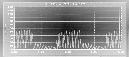
\includegraphics{img/exr-controle2.pdf}}

		Quel est le rapport i:e affiché par le Monitron ? \shortanswer{\cmh}

		Quelle est la pression moyenne inspiratoire (affichée sur le multimètre numérique du module de contrôle) ?

		\shortanswer{\cmh}
\end{exercice}

\restoregeometry
%\end{wide}

\chapter{Surveillance clinique}

\section{Données monitorées}

On retrouve à la fois des données mesurées sur le multimètre situé sur
le dessus du module de contrôle et sur le Monitron. Certaines données
sont même affichées aux deux endroits.

\emph{Il est important de noter que pour l'application du protocole de
ventilation du CHUM, c'est toujours les pressions affichées sur le
multimètre du module de contrôle que l'on doit utiliser (moyenne
inspiratoire et moyenne expiratoire).  Les pressions affichées par le Monitron (PEAK PRESSURE et PEEP/CPAP)
sont lues à la crête de l'oscillation et sont par conséquent peu
représentatives des pressions subies par les alvéoles pulmonaires.
}
\def\ptitle#1{\vspace{.4\baselineskip}\textbf{#1}\par\vspace{0.4\baselineskip}}

\begin{framed}
	\ptitle{Données affichées par le Multimètre numérique et par le Monitron. }
	\ptitle{Multimètre du module de contrôle }
	\protochum{Pression inspiratoire moyenne}\\
	\protochum{Pression expiratoire moyenne}\\
	Pression moyenne globale\\
	\protochum{Fréquence de percussion ($F_{perc}$)}

	\ptitle{Monitron}
	\raggedright
	Pression inspiratoire de crête\\
	Pression expiratoire de crête (PEP)\\
	Pression moyenne globale\\
	\protochum{Ti (convection)}\\
	\protochum{Te (convection)}\\
	I:E\\
	F\textsubscript{conv}\\
	\protochum{Fréquence de percussion ($F_{perc}$)}\\
	i:e

	\vspace{0.2\baselineskip}
	{\small *\protochum{}\space \emph{Données utilisées dans le
	protocole clinique du CHUM}}
	\end{framed}


\begin{figure}
	\newcommand{\pexp}{5}
\newcommand{\pins}{18}
\newcommand{\arrpos}{1.06}
\tikzsetnextfilename{fig-multimeter}
\begin{tikzpicture}[
		pressmark/.style={
			draw=gray,
			dashed,
		},
		pline/.style={
			pressmark,
			help lines,
			rounded corners,
			out=0,
			in=180,
			thick
			},
		pcircle/.style={
			pressmark,
			circle,
			inner sep=0.5mm,
			thick
			}
	]

	\begin{axis}[
		width=0.75\textwidth,
		height=5cm,
		name=plot,
		font=\scriptsize,
		try min ticks=6,
		xtick={0,4,8},
		ytick={0,30},
		axis x line=bottom,
		axis y line=middle,
		enlarge y limits={value=0.1, upper},
		enlarge x limits={value=0.05, upper},
		extra y ticks={5, 18},
		extra y tick labels={$P_{ins. moy.}$, $P_{exp. moy.}$},
		extra y tick style={grid=major},
		major grid style={pressmark, thick}
		]

		\addplot [
			black,
			restrict x to domain=0:8,
			] table[x=time, y=Pao] {dat/f300.dat};

		\coordinate (D) at (axis cs: \pgfkeysvalueof{/pgfplots/xmax},\pins);
		\coordinate (B) at (axis cs: \pgfkeysvalueof{/pgfplots/xmax},\pexp);

	\end{axis}

	\pic [opacity=0.99, name=mm, scale=1] at ([xshift=3.2cm, yshift=0cm]plot.east) {multimeter};

	\node [pcircle] (pmi) at (mmPmi) {\pins};
	\node [pcircle] (pme) at (mmPme) {\pexp};

	\draw [pline] (D) to (pmi);
	\draw [pline] (B) to (pme);
\end{tikzpicture}

	\caption{La pression inspiratoire moyenne et la pression expiratoire moyenne sont affichées sur me multimètre numérique se trouvant sur le dessus du ventilateur.}
\end{figure}

\section{Monitorage du rapport \ie}

On se rappellera que l'affichage du rapport \ie\ sur le Monitron n'est
fonctionnel que lorsque le Ti est plus petit que le Te. Lorsque le Ti
devient plus grand que le Te (rapport inversé), le Monitron affiche en
permanence 1\string: 1.0.

La meilleure façon de juger du rapport \ie\ est alors d'observer
l'apparence de la courbe de pression sur le monitron.

Les éléments à observer sont:

\begin{itemize}
\item
  Durée du Ti (montée de pression et plateau) versus celle du Te (chute
  de la pression) (observer à 1 ou 2 s par écran);
\item
  Présence d'un plateau. Un plateau où la pression plafonne complètement
		est suggestif d'un ratio inversé. Voir Figure~\ref{figie1}, courbe du bas.
  (observer à 1 ou 2 s par écran);
\item
  Espace sous la courbe de pression. L'augmentation de l'espace sous la
  courbe pendant l'inspiration convective est aussi suggestive d'un
  ratio inversé. Elle témoigne d'une diminution de l'amplitude des
  percussions. Voir Figure~\ref{figie8}, courbe du bas. (observer à 5 ou 8 s par
  écran);
\end{itemize}
\begin{figure*}
	\input{fig/fig-ie1}
	\caption{Rapport \ie\ adéquat (en haut) et rapport \ie\ inversé (en
	bas). On observe sur le tracé du bas un Te trop court ne permettant pas
	à la pression de redescendre entre chaque percussion. La pression
	d'équilibre est donc rapidement atteinte à la percussion suivante. Il en
	résulte une faible amplitude de variation de pression à chaque
	percussion. Vitesse de défilement à 1 s par écran.}
	\label{figie1}
	\input{fig/fig-ieimg}
	\caption{Rapport \ie\ adéquat (en haut) et rapport \ie\ inversé (en
	bas). On observe une diminution de l'amplitude de percussion sur le
	tracé du bas. Vitesse de défilement à 8 s par écran.}
	\label{figie8}
\end{figure*}

\section{Alarme}\index{alarme}

\subsection{Alarmes du module de contrôle}

\subsubsection*{Alarme du mélangeur air-oxygène}
lbs/po²
Il s'agit d'une alarme pneumatique se déclenchant lorsque le mélangeur
perd son alimentation en air ou en oxygène. Il n'y a pas de fonction
\emph{silence} ou \emph{réarmer~}: l'alarme s'arrête automatiquement
lorsque l'alimentation des deux gaz est rétablie.

\subsubsection{Alarme de surpression}\index{alarme!de surpression}

Il s'agit d'une alarme pneumatique se déclenchant lors d'une surpression
dans le module de contrôle. Son déclenchement entraine une chute de la
pression délivrée. Une fois la cause corrigée, il faut réarmer l'alarme
(bouton poussoir rouge) pour que la ventilation reprenne normalement.

Au réglage le plus sensible (rotation en sens antihoraire) l'alarme se
déclenche lorsque la pression dans le circuit avoisine les 80 \cmh.

Lorsque cette alarme se déclenche, il faut en premier lieu suspecter un
réglage inadéquat (par exemple fonction \emph{PRESSION DE CONVECTION} ou
\emph{PEP non oscillante} activées ou fréquence de percussion inférieure
à 100) ou une tubulure blanche coincée.

Il est improbable qu'une condition clinique (par exemple toux ou
résistances augmentées) entraine l'activation de cette alarme.

\subsubsection{Alarme de déconnexion}
\index{alarme!de déconnexion}

Il s'agit d'un module indépendant situé sur le côté de l'appareil et
alimenté par une batterie. Cette alarme se déclenche lorsqu'aucune
pression n'est détectée dans le circuit pour une période donnée. Cette
période peut (en théorie\ldots{}) être ajustée au moyen de la roulette
noire.

\subsection{Alarmes du Monitron}

\subsubsection*{Alarme de pression haute}%

Cette alarme se déclenche dès que la pression dans le circuit est
supérieure à la limite réglée. La valeur du réglage est indiquée par une
ligne rouge dans la zone de graphiques.

Son réglage répond même logique que l'alarme de pression haute en
ventilation conventionnelle (par exemple 10 \cmh de plus que la
pression de crête actuelle). Il faut cependant se rappeler que le
déclenchement de l'alarme n'interrompt pas la ventilation étant donné
que le Monitron et le module de contrôle sons indépendants l'un de
l'autre.

\subsubsection*{Alarme de pression basse}

Cette alarme s'active lorsque la pression dans le circuit est inférieure
au seuil réglé pour plus de 6 s (alarme visuelle) et 12 s (alarme
sonore).

Il est à noter qu'une fois la pression rétablie, l'alarme continue à
sonner tant qu'elle n'a pas été réarmée.

\section{Situations particulières}

\subsection{Obstruction de la sonde}\index{obstruction!de la sonde s'intubation}

Étant donné l'absence de monitorage du débit, il est nécessaire de faire preuve
d'une vigilance accrue afin de détecter cette complication. Une obstruction
importante de la sonde peut se manifester par :
		
\begin{itemize}
	\item Une augmentation des pressions de ventilation en l'absence de
	modification des réglages. L'augmentation de la pression à l'inspiration se
	fera de façon plus abrupte, 
	\item Une détérioration des échanges gazeux.
\end{itemize}

La perméabilité de la sonde peut être évaluée en y descendant un cathéter
d'aspiration, que ce soit en cas de doute ou sur une base régulière.  Si
l'abondance des sécrétions est problématique, le ballonnet du tube endotrachéal
peut être partiellement dégonflé pour permettre à celles-ci de remonter dans
l'oropharynx du patient. L'amplitude des percussions devra alors être réajustée
à la hausse pour compenser la fuite créée.

\begin{figure}
\centering
	\begin{tikzpicture}
		\begin{groupplot} [
				group style={
					group size=2 by 1,
					ylabels at=edge left,
				},
				ylabel=$P_{circ.} (hPa)$,
				xlabel=Temps (s),
				width=0.5\textwidth,
				restrict x to domain=1.5:4,
				ymax=40,
				every axis plot post/.style={
					mark=none
				}
			]
			\nextgroupplot [title=Résistances normales]
			\addplot [] table[x=time, y=Pao] {dat/raw5.dat};

		 \nextgroupplot [title=Résistances augmentées]
			\addplot [] table[x=time, y=Pao] {dat/raw15.dat};
		\end{groupplot}
	\end{tikzpicture}

\caption{Modification de l'apparence de la courbe de pression suite à une
augmentation des résistances. Lorsque les résistances sont normales (à gauche),
on observe une augmentation graduelle des pressions lors de l'inspiration.
Cette augmentation correspond à l'augmentation de la pression alvéolaire.
Lorsque les résistances sont élevées, les pressions sont élevées dès le début
de l'inspiration et restent stable au cours de celle-ci.}
\index{résistances!augmentées}
\end{figure}

\subsection{Fuite ou déconnexion}\index{fuite}\index{déconnexion}

Une fuite entre le phasitron et le patient ou au niveau du tube endotrachéal se
manifestera par une diminution des pressions mesurées en l'absence de
modification des réglages. La courbe de pression aura une apparence atténuée.
Une fuite dans le circuit d'humidification n’aura pas d'influence sur les
pressions de ventilations. Elle pourra, par contre, modifier la concentration
en oxygène du mélange gazeux administré au patient (appel d’air ambiant),
entrainant une hypoxémie.


%\chapter{Stratégies de ventilation}
%\chapter{Données probantes}
%\chapter{Au coeur de la bête}

%%%%%%%%%%%%%%
% Backmatter
%%%%%%%%%%%%%%

\begin{appendices}

\newgeometry{
	includeall,
	margin=0.8in,
	marginparwidth=0in,
	marginparsep=0in
}

\chapter{Protocole clinique du Centre hospitalier de l'Université de Montréal}
%\includepdf[pages=-]{../formationvdr4/documents/pub/INH-PROT-05-01.pdf}

\titleformat{\chapter}[display]{\normalfont\huge\bfseries}{\chaptertitlename\ \thechapter}{20pt}{\Huge}   
\titlespacing*{\chapter}{0pt}{-50pt}{40pt}

\chapter{Horaire type d'une formation}
\section*{Journée 1}
\begin{horaire}{450}
	\thispagestyle{empty}
	\activite{15}{Accueil des participants}
	\activite{10}{Objectifs de la formation}
	\activite{30}{Exploration des acquis}
	\activite{30}{Revue de la littérature}
	\activite{30}{Montage du circuit et vérification pré-utilisation}
	\activite{30}{Théorie relative au circuit}

	\hline
	\activite{15}{Pause}
	\hline

	\activite{30}{Paramètres de base, moniteurs et alarmes}
	\activite{45}{Position par défault et interaction i:e}
	\activite{30}{Théorie relative au rapport i:e}

	\hline
	\activite{60}{Diner}
	\hline

	\activite{40}{Évaluation du ratio i:e}
	\activite{60}{Expérimentation/théorie supplémentaire}
	\hline
	\activite{15}{Pause}
	\hline

	\activite{40}{Jeux des erreurs}
	\activite{15}{Conclusion}
\end{horaire}

\section*{Journée 2}

\begin{horaire}{450}
	\activite{60}{Retour sur la journée 1 et réponses aux questions}
	\activite{180}{Protocole de ventilation}
	\hline
	\activite{60}{Dîner}
	\hline
	\activite{180}{Mises en situations}
	\activite{15}{Conclusion}
\end{horaire}


\end{appendices}
\restoregeometry

\backmatter

\printbibliography
\printindex
\end{document}
